At \acrshort{fhict}, the \acrfull{dot} framework is required when conducting research.
This framework identifies five strategies (lab, field, showroom, library and workshop) that structure the existing information and the needs within applied research, as shown in~\cref{fig:dot_framework}. 
As applied research is about making use of existing information, this information can come from two areas (or domains), namely available work (e.i. to all existing solutions and relevant knowledge to the problem) and application domain (e.i. the context of use of the solution).
Both domains contribute to creating innovation (e.i. new solution/product).
Thus, based on the problem, the actual applied research is performed in the innovation by gathering information from the two knowledge domains to achieve the solution.
Within the innovation, a strategy/process to perform the research can be applied.
Library strategy is done to explore the theories and the current state-of-the-art solutions that could help further development.
Field strategy is done to explore the application context (end user analysis e.i. their needs, desires and limitations as organizational and physical contexts in which they will use your product). 
Lab strategy is done to learn if chosen concepts and solutions of the final product work or to test different scenarios.
Showroom strategy is done to compare existing work.
Finally, workshop strategy is done to explore opportunities (e.i. prototyping, designing and co-creation activities)~\cite{dot}. Each of the five strategies decide on the research method that best fits the need. These needs have to fit completeness, certainty, relevance and rigor.
The method depends on your specific research question and the \acrshort{ict} field. 
Each field has its own methods, from which the most important are listed in~\cref{fig:dot_methods}.
\begin{figure}[h]
    \centering
    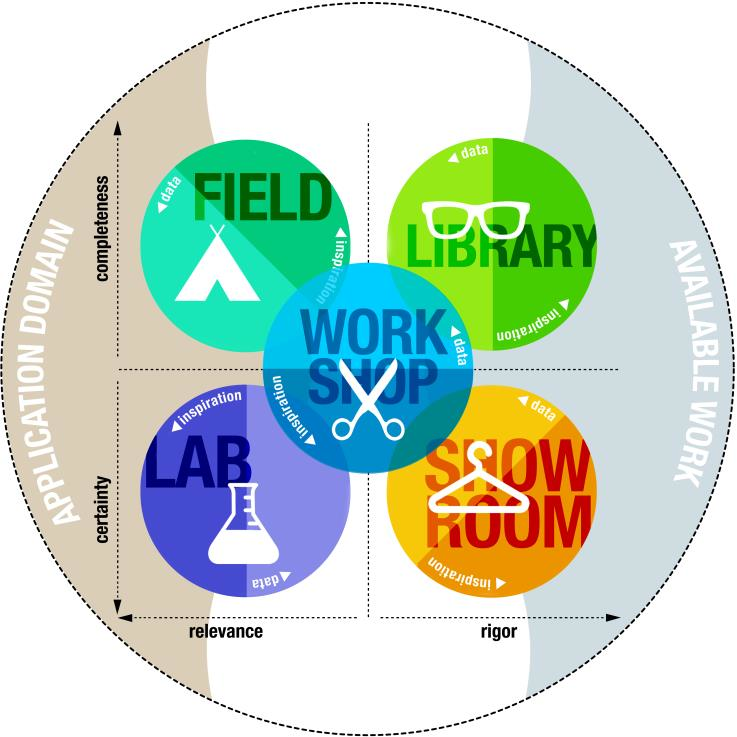
\includegraphics[width=0.48\textwidth]{figures/DOT-framework.png}
    \caption{Graphical representation of the \acrfull{dot} framework (source: \url{http://ictresearchmethods.nl/The_DOT_Framework})}
    \label{fig:dot_framework}
\end{figure}
\begin{figure}[h]
    \centering
    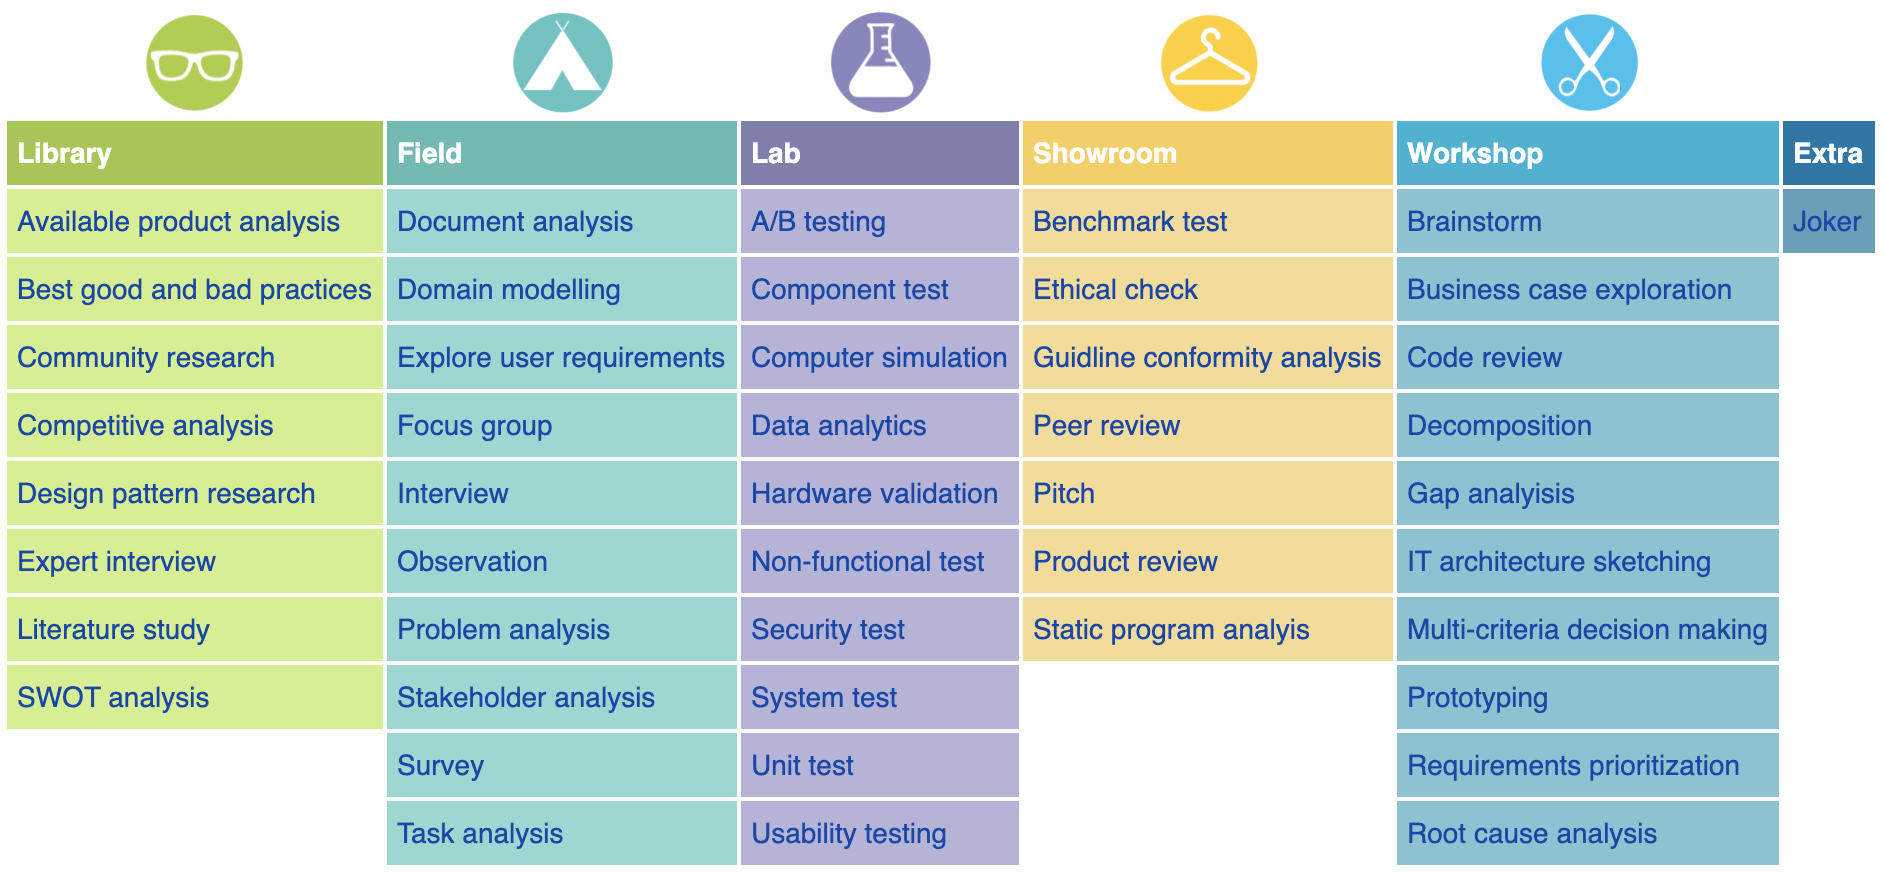
\includegraphics[width=\textwidth]{figures/dot_methods.png}
    \caption{\acrshort{dot} framework methods (source: \url{http://ictresearchmethods.nl/Methods})}
    \label{fig:dot_methods}
\end{figure}

\noindent Students are required to apply the \acrshort{dot} framework throughout their study at \acrshort{fhict}, especially when doing the internship and graduation. The following section describes the supervision of research during internship.